\section{Funktionen}
\subsection{Symetrien}
\begin{itemize}
    \item Eine Funktion $f$ heisst gerade, wenn $f(-x) = f(x)$ für alle $x \in D$.\\\\
    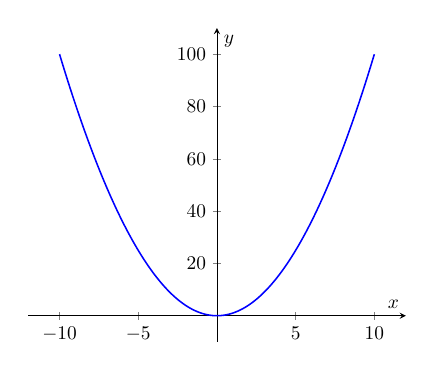
\begin{tikzpicture}[scale=0.7]
        \begin{axis}[
            axis lines = middle,
            xlabel = $x$,
            ylabel = $y$,
            enlargelimits]
            \addplot[domain = -10:10,
            samples = 200,
            smooth,
            thick,
            blue] {x^2};
        \end{axis}
    \end{tikzpicture}
    \item Eine Funktion $f$ heisst ungerade, wenn $f(-x) = -f(x)$ für alle $x \in D$.\\\\
    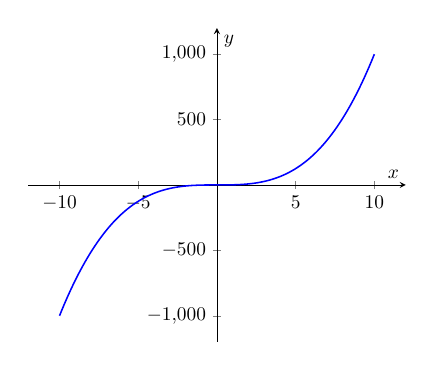
\begin{tikzpicture}[scale=0.7]
        \begin{axis}[
            axis lines = middle,
            xlabel = $x$,
            ylabel = $y$,
            enlargelimits]
            \addplot[domain = -10:10,
            samples = 200,
            smooth,
            thick,
            blue] {x^3};
        \end{axis}
    \end{tikzpicture}
\end{itemize}
\subsection{Umkehrfunktionen}
Für die Umkehrfunktionen einfach nach x auflösen und dann x und y vertauschen.\\
Eigenschaften von Umkehrfunktionen:
\begin{itemize}
    \item Für jede Relation R gilt $R^{-1^{-1}} = R$
    \item R ist genau dann linksvollständig, wenn $R^{-1}$ rechtseindeutig ist.
    \item R ist genau dann linkseindeutig, wenn $R^{-1}$ rechtseindeutig ist.
\end{itemize}
\subsection{Komposition}
Für $g: A \rightarrow B $ und $f: B \rightarrow C$ definieren wir:
\begin{align*}
    f \circ g: A \rightarrow C
\end{align*}
\begin{align*}
    (f \circ g)(x) = f(g(x))
\end{align*}
Wörtlich sagt man auch ''f nach g'' da f nach g ausgeführt wird bzw. g zuerst ausgeführt wird.
\subsubsection{Assoziativität}
Für $f: A \rightarrow B$, $g: B \rightarrow C$ und $h: C \rightarrow D$ gilt:
\begin{itemize}
    \item $(f \circ g) \circ h = f \circ (g \circ h)$
\end{itemize}
\subsection{Summenformel}
Arithmetische Summenformel:
\begin{align*}
    \sum_{i=1}^{n} i = \frac{n(n+1)}{2}
\end{align*}
Summe der Quadratzahlen:
\begin{align*}
    \sum_{i=1}^{n} i^2 = \frac{n(n+1)(2n+1)}{6}
\end{align*}
\subsection{Betragsfunktion}
\begin{center}
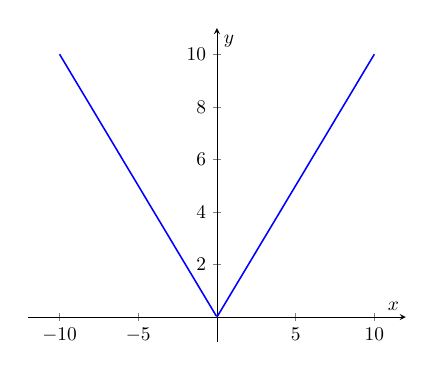
\begin{tikzpicture}[scale=0.7]
    \begin{axis}[
        axis lines = middle,
        xlabel = $x$,
        ylabel = $y$,
        enlargelimits]
        \addplot[domain = -10:10,
        samples = 200,
        smooth,
        thick,
        blue] {abs(x)};
    \end{axis}
\end{tikzpicture}
\end{center}
\begin{align*}
    |x| = \begin{cases}
        x & \text{für } x \geq 0\\
        -x & \text{für } x < 0
    \end{cases}
\end{align*}